\documentclass[11pt]{beamer}
\usepackage[UTF8]{ctex}
%\usepackage[utf8]{inputenc}
%\usepackage[T1]{fontenc}
%\usepackage{lmodern}
%\usepackage{amsmath}
%\usepackage{amsfonts}
%\usepackage{amssymb}
\usepackage{graphicx}
\usetheme{CambridgeUS}

%%% 超链接
\usepackage[]{hyperref}

\usepackage{pdfpages}

%%% UML
\usepackage[simplified]{pgf-umlcd}

%%%%%  代码
\usepackage{listings}\usepackage{color}  
\definecolor{dkgreen}{rgb}{0,0.6,0}  
\definecolor{gray}{rgb}{0.5,0.5,0.5}  
\definecolor{mauve}{rgb}{0.58,0,0.82}  

\lstset{ %  
	basicstyle=\ttfamily,
	%basicstyle=\footnotesize,           % the size of the fonts that are used for the code  
	numbers=left,                   % where to put the line-numbers  
	numberstyle=\tiny\color{gray},  % the style that is used for the line-numbers  
	stepnumber=1,                   % the step between two line-numbers. If it's 1, each line   
	% will be numbered  
	numbersep=5pt,                  % how far the line-numbers are from the code  
	backgroundcolor=\color{white},      % choose the background color. You must add \usepackage{color}  
	showspaces=false,               % show spaces adding particular underscores  
	showstringspaces=false,         % underline spaces within strings  
	showtabs=false,                 % show tabs within strings adding particular underscores  
	frame=single,                   % adds a frame around the code  
	rulecolor=\color{black},        % if not set, the frame-color may be changed on line-breaks within not-black text (e.g. commens (green here))  
	tabsize=2,                      % sets default tabsize to 2 spaces  
	captionpos=b,                   % sets the caption-position to bottom  
	breaklines=true,                % sets automatic line breaking  
	breakatwhitespace=false,        % sets if automatic breaks should only happen at whitespace  
	% title=\lstname,                   % show the filename of files included with \lstinputlisting;  
	% also try caption instead of title  
	keywordstyle=\color{blue},          % keyword style  
	commentstyle=\color{dkgreen},       % comment style  
	stringstyle=\color{mauve},         % string literal style  
	escapeinside={\%*}{*)},            % if you want to add LaTeX within your code  
	morekeywords={*,...}               % if you want to add more keywords to the set  
}  

% 分栏-用于目录
\usepackage{multicol}


%%%%%表格
\usepackage{longtable}
\usepackage{subfigure}
\usepackage{booktabs}

%%%%%
%\usepackage[backend=bibtex,sorting=none]{biblatex}
%\addbibresource{reference.bib} %BibTeX数据文件及位置
%\setbeamerfont{footnote}{size=\tiny} 
%\setbeamertemplate{bibliography item}[text]

%%% 参考文献
\usepackage{natbib}

%% LOGO放右上
\setbeamertemplate{frametitle}
{\begin{beamercolorbox}[wd=\paperwidth]{frametitle}
		\strut\hspace{0.5em}\insertframetitle\strut
		\hfill
		\raisebox{-2mm}{
\includegraphics[width=1cm]{figures/HNUC.jpeg}}
	\end{beamercolorbox}
}

%%% 课件属性定义
\author{郭泰彪}
\title{区块链原理及应用}
\subtitle{第5课:区块链密码学基础(实验)}
\institute[湖工商大数据研究院]{湖南工商大学大数据与互联网创新研究院}
\date{2020年10月10日}
\titlegraphic{
\includegraphics[width=2cm]{figures/HNUC.jpeg}}


\begin{document}
\begin{frame}[plain]
	\maketitle
\end{frame}

\begin{frame}
	\frametitle{目录}
	\begin{multicols}{2}
		\tableofcontents[sectionstyle=show,subsectionstyle=show/shaded]
	\end{multicols}
\end{frame}

\section{区块链密码学基础回顾}

\begin{frame}{哈希( hash)函数}
	\begin{minipage}[t]{0.5\linewidth}
		\begin{itemize}
			\item \textbf{单向性}
			
			{\scriptsize 即给定一个输入数,容易计算出它的哈希值,但是已知一个哈希值根据同样的算法不能得到原输入数}。
			
			\item \textbf{弱抗碰撞性}
			
			{\scriptsize 即给定一个输入数,要找到另一个得到给定数的哈希值,在使用同一种方法时,在计算上不可行。}
			
			\item \textbf{强抗碰撞性}
			
			{\scriptsize 即对于任意两个不同的输入数,根据同样的算法计算出相同的哈希值,在计算上不可行}。
		\end{itemize}
	\end{minipage}%
	\begin{minipage}[t]{0.5\linewidth}
	\begin{figure}
		\centering
		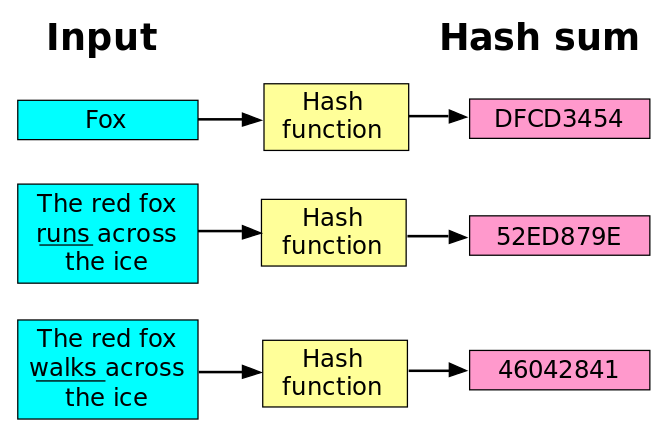
\includegraphics[width=0.7\linewidth]{figures/Hashfunction}
		\label{fig:hashfunction}
	\end{figure}
\end{minipage}%
\end{frame}

\begin{frame}{哈希函数在区块链的应用}
	\begin{multicols}{2}
		\begin{itemize}
			\item \textbf{地址生成}
			
			{\tiny 散列函数在区块链中被用于地址生成。例如以太坊中,地址是由名为Keccak-256的散列函数对私钥计算得出的。又例如比特币中,地址是由SHA256和RIPEMD160得出。比特币中的散列函数必须考虑防碰撞性,否则不同用户间地址会冲突。}
			
			\item \textbf{交易签名}
			
			{\tiny 散列函数常用来构造数字签名,数字签名类似签署一张支票,签名可信度确保了支票的有效性。数字签名是由私钥和需要被签名的数据散列而生成,签名可以进行签名者身份识别和抗抵赖,数字签名在区块链中被用于确保交易和区块的签名验证。}
			
			\item \textbf{区块校验}
			
			{\tiny 区块链中的区块是由区块对应的散列值确定,散列函数在其中充当了鉴别和完整性校验的双重角色。节点在接受一个新的区块后,只需要验证散列值就可以确保区块未被篡改。}
			
			\item \textbf{设计共识算法}
			
			{\tiny 对于利用PoW(Proof of Work,工作量证明)的区块链系统来说,散列函数还会被用于共识算法。}
			
			\item \textbf{默克尔树(Merkle Tree)}
			
			\item \textbf{布隆过滤器(Bloom Filter)}
		\end{itemize}
	\end{multicols}
\end{frame}

\section{实验环境的准备-云端}
\subsection{实验环境的准备-云端-katacoda}
\begin{frame}
	\frametitle{katacoda}
	\begin{enumerate}
		\item 注册github:
		
		github.com
		\item 新建docker云实例:
		
		www.katacoda.com/courses/docker/playground
	\end{enumerate}

\end{frame}
\subsection{检查docker是否成功安装}
\begin{frame}[fragile]
	\frametitle{检查docker是否成功安装}
	在命令行中执行下面的语句:
	\begin{lstlisting}[language=sh,numbers=none]
docker version
\end{lstlisting}
	
	若显示类似输出则表示成功安装:
\begin{lstlisting}[language=sh,linerange={1-18},basicstyle=\fontsize{6}{8}\ttfamily]
docker version
Client:
Version:           19.03.8
API version:       1.40
Go version:        go1.13.8
Git commit:        afacb8b7f0
Built:             Tue Jun 23 22:26:12 2020
OS/Arch:           linux/amd64
Experimental:      false

Server:
Engine:
Version:          19.03.8
API version:      1.40 (minimum version 1.12)
Go version:       go1.13.8
Git commit:       afacb8b7f0
Built:            Thu Jun 18 08:26:54 2020
OS/Arch:          linux/amd64
Experimental:     false
containerd:
Version:          1.3.3-0ubuntu2
GitCommit:        
runc:
Version:          spec: 1.0.1-dev
GitCommit:        
docker-init:
Version:          0.18.0
GitCommit:        
\end{lstlisting}
\end{frame}

\subsection{运行HelloWorld}
\begin{frame}[fragile]
	\frametitle{运行HelloWorld}
	在命令行中执行下面的语句运行简单区块链:
	\begin{lstlisting}[language=sh,numbers=none,basicstyle=\fontsize{7}{9}\ttfamily]
docker run --rm registry.cn-shenzhen.aliyuncs.com/blockchain101/hello_blockchain
\end{lstlisting}
输出结果:
	\begin{lstlisting}[language=sh,basicstyle=\fontsize{6}{8}\ttfamily]
/$$       /$$                     /$$                 /$$                 /$$          
| $$      | $$                    | $$                | $$                |__/          
| $$$$$$$ | $$  /$$$$$$   /$$$$$$$| $$   /$$  /$$$$$$$| $$$$$$$   /$$$$$$  /$$ /$$$$$$$ 
| $$__  $$| $$ /$$__  $$ /$$_____/| $$  /$$/ /$$_____/| $$__  $$ |____  $$| $$| $$__  $$
| $$  \ $$| $$| $$  \ $$| $$      | $$$$$$/ | $$      | $$  \ $$  /$$$$$$$| $$| $$  \ $$
| $$  | $$| $$| $$  | $$| $$      | $$_  $$ | $$      | $$  | $$ /$$__  $$| $$| $$  | $$
| $$$$$$$/| $$|  $$$$$$/|  $$$$$$$| $$ \  $$|  $$$$$$$| $$  | $$|  $$$$$$$| $$| $$  | $$
|_______/ |__/ \______/  \_______/|__/  \__/ \_______/|__/  |__/ \_______/|__/|__/  |__/
/$$    /$$$$$$    /$$                                  
/$$$$   /$$$_  $$ /$$$$                                  
|_  $$  | $$$$\ $$|_  $$                                  
| $$  | $$ $$ $$  | $$                                  
| $$  | $$\ $$$$  | $$                                  
| $$  | $$ \ $$$  | $$                                  
/$$$$$$|  $$$$$$/ /$$$$$$                                
|______/ \______/ |______/                                
\end{lstlisting}
\end{frame}

% 20分钟
\section{Python语言速览}
\subsection{人生苦短,我用Python}
\begin{frame}{人生苦短,我用Python}
	Python简洁却强大、简单却专业,它是当今世界最受欢迎的编程语言,学好它终身受用。\footnote{\href{http://www.icourse163.org/course/BIT-268001}{国家精品课程:Python语言程序设计}}
	\begin{multicols}{2}
		\begin{itemize}
			\item	Python 是流行语言
			\item	Python 是入门语言
			\item	Python 是玩具语言
			\item	Python 是胶水语言
			\item	Python 是黑客语言
			\item	Python 是通用语言
		\end{itemize}
	\end{multicols}
\end{frame}

\begin{frame}{Python应用领域}
	\begin{figure}
		\centering
		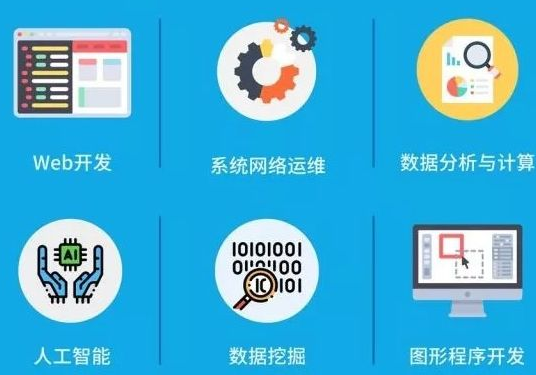
\includegraphics[width=0.8\linewidth]{figures/python-field}
		\label{fig:python-field}
	\end{figure}
\end{frame}

\begin{frame}[allowframebreaks]{\#潘石屹用Python解决100个问题\#}
	微博话题:\textbf{\#潘石屹用Python解决100个问题\#}\cite{panshiyi100}

	2019年,当地产大佬潘石屹要把学习Python作为生日礼物送给自己的时候,微博上还多是一阵调侃之声,2020年潘同学已经在Python考试中得到99分的好成绩。时年56岁的小潘同学要再一次抓住“青春”的尾巴。
	\begin{figure}
		\centering
		
\includegraphics[width=0.7\linewidth]{figures/pythonPanshiyi01}
		\label{fig:pythonpanshiyi01}
	\end{figure}

	\begin{figure}
		\centering
		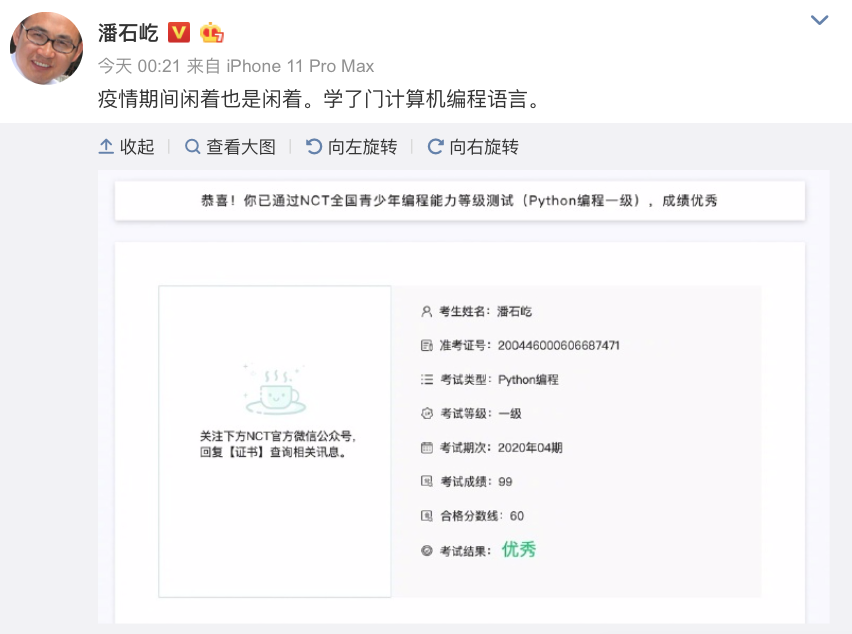
\includegraphics[width=0.8\linewidth]{figures/pythonPanshiyi03}
		\label{fig:pythonpanshiyi03}
	\end{figure}
\end{frame}

\begin{frame}{潘石屹谈为什么学Python}
	\begin{figure}
		\centering
		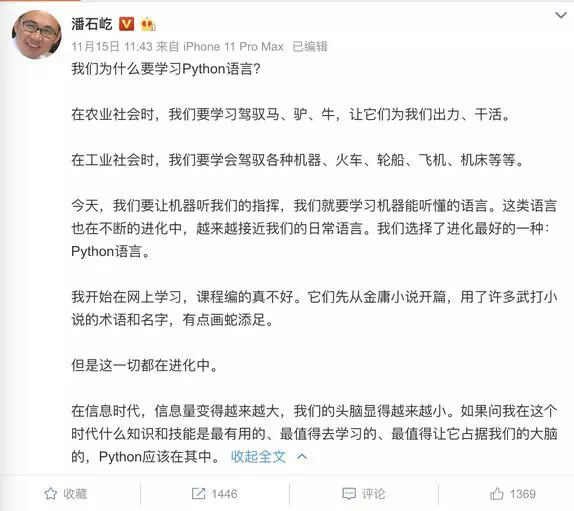
\includegraphics[width=0.6\linewidth]{figures/pythonPanshiyi02}
		\label{fig:pythonpanshiyi02}
	\end{figure}
\end{frame}

\subsection{代码格式}

% lstlisting报错问题解决思路:http://blog.sina.com.cn/s/blog_5e16f1770102dxps.html
\begin{frame}[fragile]
	\frametitle{代码格式}

	\begin{minipage}[t]{0.5\linewidth}
		\begin{itemize}
			\item Python是一门脚本语言,可以一行行输入并立即执行;
			\item Python也可以将代码保存到文件中,以\textbf{类}、\textbf{函数}等方式对代码进行组织。
		\end{itemize}
	\end{minipage}%
	% 此行用于空格
	\begin{minipage}[t]{0.05\linewidth}
		\quad
	\end{minipage}%
	\begin{minipage}[t]{0.4\linewidth}
		\begin{figure}
			\lstinputlisting[language=Python,basicstyle=\scriptsize ,title=python代码基本结构\cite{rossum1995python}]{./figures/basicpython.py}
		\end{figure}
	\end{minipage}%
\end{frame}

\subsection{Python的基本语法}
\begin{frame}[fragile]
	\frametitle{类}
	\begin{minipage}[t]{0.5\linewidth}
		\begin{itemize}
			\item 类可以用来对代码进行组织和管理;
			\item 类可以对现实世界的对象进行抽象和建模;
			\item 类的基本组成包含属性和方法;
			\item 类支持继承等面向对象编程的功能;
		\end{itemize}

		例子
		\begin{itemize}
			\item 类名: 人类(human)
			\item 属性:体重 (weight),年龄 (age),性别(sex);
			\item 方法:吃(eat), 睡(sleep), 玩(play);
		\end{itemize}
	\end{minipage}%
	% 此行用于空格
	\begin{minipage}[t]{0.05\linewidth}
		\quad
	\end{minipage}%
	\begin{minipage}[t]{0.4\linewidth}
		\begin{figure}
			\lstinputlisting[language=Python,basicstyle=\scriptsize ,title=python定义人类]{./figures/classhuman.py}
		\end{figure}
	\end{minipage}
\end{frame}

\begin{frame}[fragile]
	\frametitle{函数}
	\begin{minipage}[t]{0.4\linewidth}
		\begin{itemize}
			\item 不属于任何类的"方法",没有self参数
			\item 函数内包含具体逻辑
		\end{itemize}
	\end{minipage}%
	\begin{minipage}[t]{0.05\linewidth}
		\quad 	% 此行用于空格
	\end{minipage}%
	\begin{minipage}[t]{0.5\linewidth}
		\lstinputlisting[language=Python,basicstyle=\scriptsize,linerange={1-4}]{./figures/func.py}

		\lstinputlisting[language=Python,basicstyle=\scriptsize,linerange={6-17}]{./figures/func.py}
	\end{minipage}
\end{frame}

\begin{frame}[fragile]
	\frametitle{具体逻辑-(Python内置类+用户定义)}
	% 此行用于空格
	\begin{minipage}[t]{0.25\linewidth}
		判断语句:
		\begin{itemize}
			\item 条件语句
			\item 循环语句
		\end{itemize}
	\end{minipage}%
	\begin{minipage}[t]{0.25\linewidth}
		运算符:
		\begin{itemize}
			\item 算术运算符
			\item  比较运算符
			\item 赋值运算符
			\item 逻辑运算符
			\item ...
		\end{itemize}
	\end{minipage}%
	\begin{minipage}[t]{0.25\linewidth}
		复杂数据结构:
		\begin{itemize}
			\item 字符串
			\item 列表
			\item 元组
			\item 字典
		\end{itemize}
	\end{minipage}%
	\begin{minipage}[t]{0.25\linewidth}
		用户定义:
		\begin{itemize}
			\item 变量
			\item 自定义函数
			\item 自定义类
		\end{itemize}
	\end{minipage}
\end{frame}

\begin{frame}{关键字}
	\scriptsize
	\begin{multicols}{3}
		\textbf{and}	逻辑运算符。

		\textbf{as}	创建别名。

		\textbf{assert}	用于调试。

		\textbf{break}	跳出循环。

		\textbf{class}	定义类。

		\textbf{continue}	继续循环的下一个迭代。

		\textbf{def}	定义函数。

		\textbf{del}	删除对象。

		\textbf{elif}	在条件语句中使用,等同于 else if。

		\textbf{else}	用于条件语句。

		\textbf{except}	处理异常,发生异常时如何执行。

		\textbf{False}	布尔值,比较运算的结果。

		\textbf{finally}	处理异常异常,都将执行一段代码。

		\textbf{for}	创建 for 循环。

		\textbf{from}	导入模块的特定部分。

		\textbf{global}	声明全局变量。

		\textbf{if}	写一个条件语句。

		\textbf{import}	导入模块。

		\textbf{in}	检查列表、元组等集合中是否存在某个值。

		\textbf{is}	测试两个变量是否相等。

		\textbf{lambda}	创建匿名函数。

		\textbf{None}	表示 null 值。

		\textbf{nonlocal}	声明非局部变量。

		\textbf{not}	逻辑运算符。

		\textbf{or}	逻辑运算符。

		\textbf{pass}	null 语句,一条什么都不做的语句。

		\textbf{raise}	产生异常。

		\textbf{return}	退出函数并返回值。

		\textbf{True}	布尔值,比较运算的结果。

		\textbf{try}	编写 try...except 语句。

		\textbf{while}	创建 while 循环。

		\textbf{with}	用于简化异常处理。

		\textbf{yield}	结束函数,返回生成器。
	\end{multicols}
\end{frame}

\begin{frame}[fragile]
	\frametitle{判断语句}
	\begin{minipage}[t]{0.5\linewidth}
		\begin{itemize}
			\item	条件语句:
			      \begin{itemize}
				      \item if else判断
			      \end{itemize}
			\item 循环语句:
			      \begin{itemize}
				      \item while循环
				      \item for循环
				      \item 中断循环标志:break,continue,pass
			      \end{itemize}
		\end{itemize}
	
			\begin{figure}
		\centering
		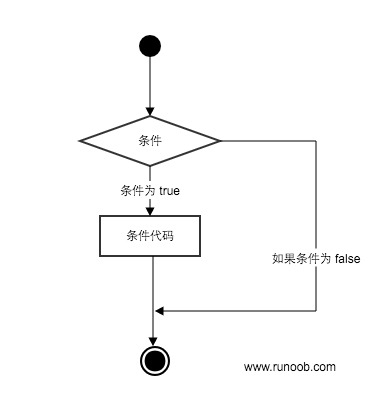
\includegraphics[height=0.35\textheight]{figures/ifelse}
		\label{fig:ifelse}
	\end{figure}
	\end{minipage}%
	% 此行用于空格
	\begin{minipage}[t]{0.05\linewidth}
		\quad
	\end{minipage}%
	\begin{minipage}[t]{0.4\linewidth}
\begin{figure}
	\centering
	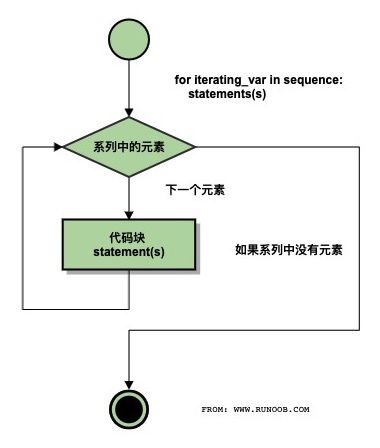
\includegraphics[height=0.35\textheight]{figures/forloop}
	\label{fig:forloop}
\end{figure}	

\begin{figure}
	\centering
	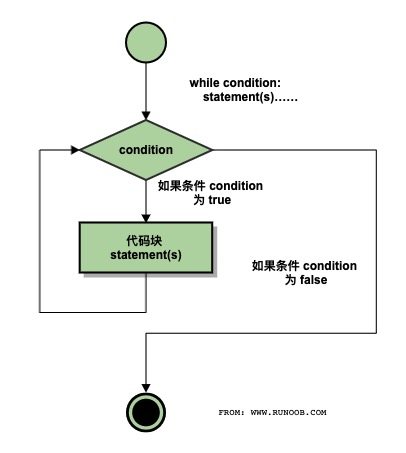
\includegraphics[height=0.35\textheight]{figures/whileloop}
	\label{fig:whileloop}
\end{figure}
	\end{minipage}
\end{frame}

\begin{frame}[fragile]
	\frametitle{运算符}
	\begin{minipage}[t]{0.33\linewidth}
		算数运算符:

		\begin{tabular}{|c|c|}
			\hline
			+   & 简单赋值 \\
			\hline
			-   & 加法赋值 \\
			\hline
			*   & 减法赋值 \\
			\hline
			/   & 乘法赋值 \\
			\hline
			\%  & 除法赋值 \\
			\hline
			**= & 取模赋值 \\
			\hline
			//  & 幂赋值   \\
			\hline
		\end{tabular}
	\end{minipage}%
	\begin{minipage}[t]{0.33\linewidth}
		赋值运算符:

		\begin{tabular}{|c|c|}
			\hline
			=   & 简单赋值   \\
			\hline
			+=  & 加法赋值   \\
			\hline
			-=  & 减法赋值   \\
			\hline
			*=  & 乘法赋值   \\
			\hline
			/=  & 除法赋值   \\
			\hline
			\%= & 取模赋值   \\
			\hline
			**= & 幂赋值     \\
			\hline
			//= & 取整除赋值 \\
			\hline
		\end{tabular}
	\end{minipage}%
	\begin{minipage}[t]{0.33\linewidth}
		比较运算符:

		\begin{tabular}{|c|c|}
			\hline
			== & 等于     \\
			\hline
			!= & 不等于   \\
			\hline
			>  & 大于     \\
			\hline
			<  & 小于     \\
			\hline
			>= & 大于等于 \\
			\hline
			<= & 小于等于 \\
			\hline
		\end{tabular}
	\end{minipage}
\end{frame}

\begin{frame}[fragile]
	\frametitle{复杂数据结构}
		\begin{itemize}
			\item 元组
			\begin{lstlisting}[numbers=none]
('physics', 'chemistry', 1997, 2000)
\end{lstlisting}
			\item 列表
			\begin{lstlisting}[numbers=none]
['physics', 'chemistry', 1997, 2000]
\end{lstlisting}
			\item 字典
			\begin{lstlisting}[numbers=none]
{key1 : value1, key2 : value2 }
\end{lstlisting}
			\item 字符串
			\begin{lstlisting}[numbers=none]
'Hello World!'
\end{lstlisting}
		\end{itemize}
\end{frame}

%\begin{frame}[fragile]
%	\frametitle{title}
%	\begin{minipage}[t]{0.5\linewidth}
%		\begin{itemize}
%			\item	dosomething
%		\end{itemize}
%	\end{minipage}%
%	% 此行用于空格
%	\begin{minipage}[t]{0.05\linewidth}
%		\quad
%	\end{minipage}%
%	\begin{minipage}[t]{0.4\linewidth}
%		\begin{figure}
%			\lstinputlisting[language=Python,basicstyle=\scriptsize ,title=python定义人类]{./figures/classhuman.py}
%		\end{figure}
%	\end{minipage}
%\end{frame}

\subsection{更多Python资料}
\begin{frame}[fragile]
	\frametitle{更多Python资料}

	\begin{itemize}
		\item 	视频教程:
		      \begin{itemize}
			      \item \href{http://www.icourse163.org/course/BIT-268001}{\underline{北理工Python程序设计系列}}
		      \end{itemize}

		\item 	书籍:
		      \begin{itemize}
			      \item \href{https://item.jd.com/12279949.html}{\underline{Python基础教程(第三版)}}
		      \end{itemize}

		\item 	开发工具:
		      \begin{itemize}
			      \item \href{https://www.jetbrains.com/pycharm/}{\underline{PyCharm}}:一个智能化的Python 开发环境
			      \item \href{https://www.anaconda.com/products/individual}{\underline{conda}} :集成了很多Python数据分析工具的Python解决方案
		      \end{itemize}

		\item 	Python项目:
		      \begin{itemize}
			      \item \href{https://github.com/vinta/awesome-python}{\underline{awesome-python}}:包含众多优秀Python项目
		      \end{itemize}
	\end{itemize}

	{\small 点击可以\textbf{资料名称}可以直达下载地址}。
\end{frame}

\section{实验任务}
% 实现一个简单区块链,其中每个区块都指向上一个区块。
%这是一个区块链的基本的实现,不包含工作证明或点对点等高级功能。区块链功能的基本实现,可以通过动作集对区块链进行操作。
%运行成功后按照提示进行操作即可。
\subsection{实验任务介绍}
\begin{frame}{实验任务说明-简单区块链}
\begin{figure}
	\centering
	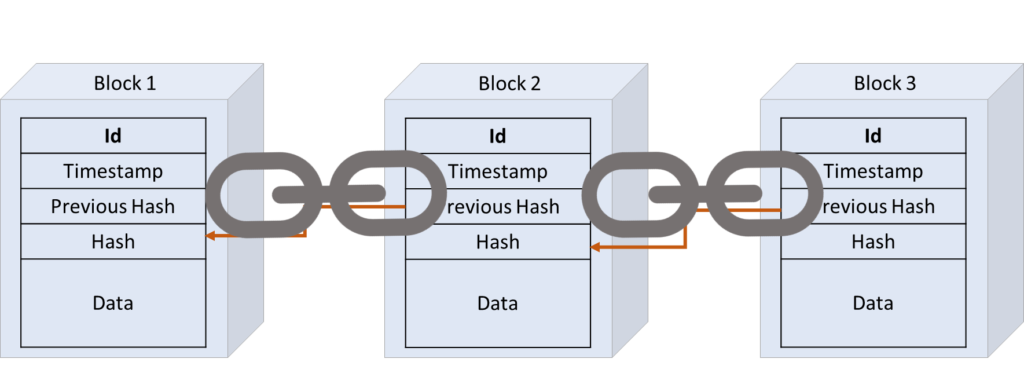
\includegraphics[width=0.7\linewidth, height=0.3\textheight]{figures/blockchain}
	\label{fig:blockchain}
\end{figure}
		\scriptsize
	\begin{multicols}{2}
			\begin{itemize}
			\item 包括:
			\begin{itemize}
				\item 将消息按照顺序打包成区块;
				\item 将区块按照顺序链接成区块链;
				\item 能够验证区块链是否被破坏:
				\begin{itemize}
					\item 能够验证消息是否被破坏;
					\item 能够验证区块是否被破坏;
				\end{itemize}
				\item 命令行的操作界面;
			\end{itemize}
			\item 不包括:
			\begin{itemize}
				\item 不包含数字签名等认证功能等实现;
				\item 工作量证明等共识算法的实现;
				\item 点对点通信等分布式系统的实现;
			\end{itemize}
		\end{itemize}
	\end{multicols}
\end{frame}

\begin{frame}{实验任务说明-简单区块链}
	\begin{figure}
		\centering
		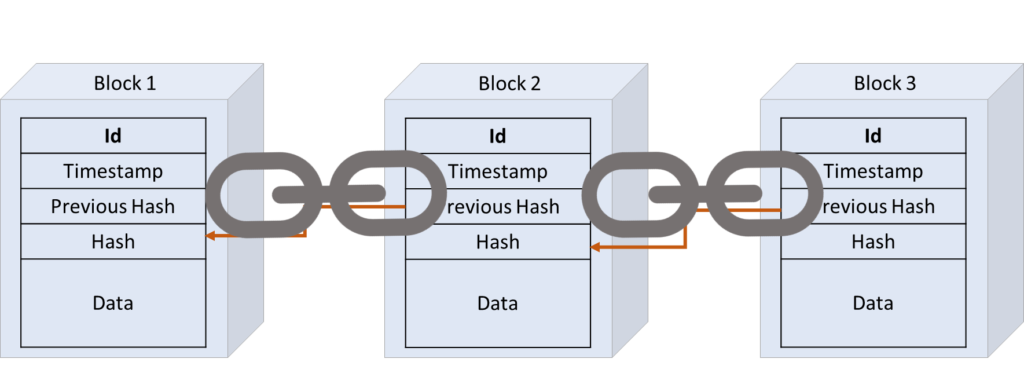
\includegraphics[width=0.9\linewidth]{figures/blockchain}
		\label{fig:blockchain}
	\end{figure}
\end{frame}

\subsection{任务分析-消息Message}
\begin{frame}{任务分析-消息Message}
	消息(Message)将用户的数据按顺序排列好,准备打包成区块。
	\begin{itemize}
		\item 功能:
		\begin{itemize}
			\item 将消息按照顺序打包
			\item 能够验证消息是否被破坏
		\end{itemize}
		\item 属性:
		\item 方法:
		\begin{itemize}
			\item  链接(link):将消息按照时间顺序链接起来
			
			\item 生成消息哈希(seal):
			
			$hash_{message}=sha256(hash_{prev} + hash_{payload})$
			
			\item 验证消息的完整性(Validate):
			
		 再次计算$hash_{message}=sha256(hash_{prev} + hash_{payload})$,验证hash是否相同
		\end{itemize}
	\end{itemize}
\end{frame}

\subsection{任务分析-区块Block}
\begin{frame}{任务分析-区块Block}
	区块(Block)是将一组消息打包好,并根据前一个区块的哈希生成新的区块。
	\begin{itemize}
		\item 功能:
		\begin{itemize}
			\item 将区块按照顺序链接成区块链
			\item 能够验证区块是否被破坏
		\end{itemize}
		\item 属性:
		\item 方法:
		\begin{itemize}
			\item  链接(link):将消息按照时间顺序链接起来
			\item 生成消息哈希(seal):
			遍历消息列表,生成$hash_{block}=sha256(hash_{prev} + timestamp + hash_{message[-1]})$
			\item 验证区块的完整性(Validate):
			
			验证每个消息的哈希,然后验证链的完整性,最后验证块的哈希。
		\end{itemize}
	\end{itemize}
\end{frame}

\subsection{任务分析-简单区块链SimpleChain}
\begin{frame}{任务分析-简单区块链SimpleChain}
	简单区块链(SimpleChain)将区块链接起来
	\begin{itemize}
		\item 功能:
		\begin{itemize}
			\item 链接区块生成区块链
		\end{itemize}
		\item 属性:
		\item 方法:
		\begin{itemize}
			\item 添加区块:添加被验证有效的区块

			\item 验证区块链的完整性(validate):依次验证每个区块,无效的区块会让链失效
		\end{itemize}
	\end{itemize}
\end{frame}

\subsection{任务分析-业务逻辑}
\begin{frame}{任务分析-业务逻辑}
	业务逻辑是我们如何操作简单区块链的逻辑
	\begin{itemize}
		\item 功能:根据输入的数字来完成录入消息、生成区块等操作
		\item 属性:
		\item 方法:
		\begin{itemize}
			\item 将现有块添加到链
			
			\item 显示整个区块链
			
			\item 显示一个区块
			
			\item 验证区块链的完整性
			
			\item 退出程序
		\end{itemize}
	\end{itemize}
\end{frame}

\section{简单区块链的定义和实现}

\begin{frame}
	\frametitle{简单区块链的模型总览}
	\begin{figure}
			\begin{center}
			\scriptsize\ttfamily
			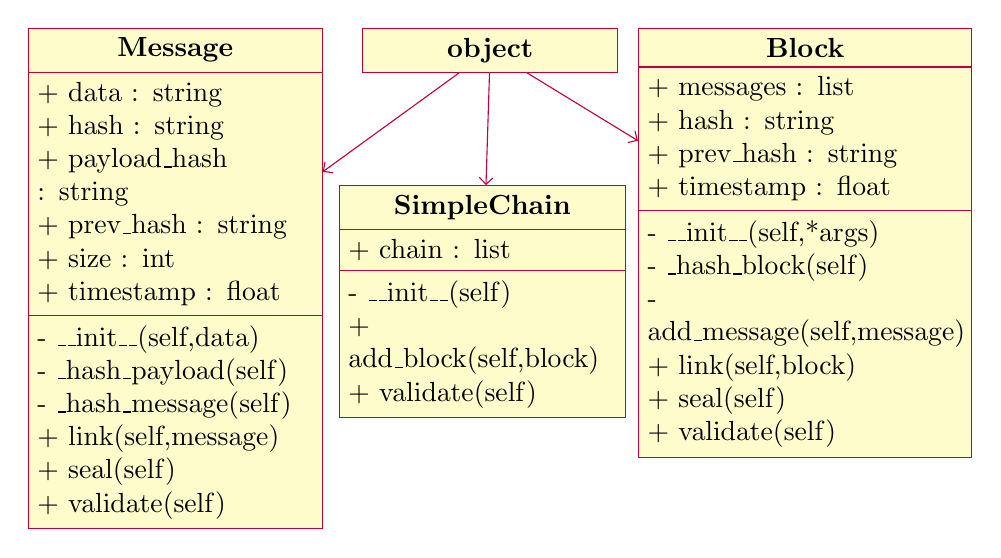
\begin{tikzpicture}
			\begin{class}[text width = 3.5cm]{Message}{0, 0}
			\attribute{+ data : string}
			\attribute{+ hash : string}
			\attribute{+ payload\_hash : string}
			\attribute{+ prev\_hash : string}
			\attribute{+ size : int}
			\attribute{+ timestamp : float}
			
			\operation{- \_\_init\_\_(self,data)}
			\operation{- \_hash\_payload(self)}
			\operation{- \_hash\_message(self)}
			\operation{+ link(self,message)}
			\operation{+ seal(self)}
			\operation{+ validate(self)}
			\end{class}
			
			\begin{class}[text width = 3cm]{object}{4, 0}
			\end{class}
			
			\begin{class}[text width = 4cm]{Block}{8, 0}
			\attribute{+ messages : list}
			\attribute{+ hash : string}
			\attribute{+ prev\_hash : string}
			\attribute{+ timestamp : float}
			
			\operation{- \_\_init\_\_(self,*args)}
			\operation{- \_hash\_block(self)}
			\operation{- add\_message(self,message)}
			\operation{+ link(self,block)}
			\operation{+ seal(self)}
			\operation{+ validate(self)}
			\end{class}
			
			\begin{class}[text width = 3.4cm]{SimpleChain}{3.9, -2}
			\attribute{+ chain : list}
			
			\operation{- \_\_init\_\_(self)}
			\operation{+ add\_block(self,block)}
			\operation{+ validate(self)}
			\end{class}
			
			\unidirectionalAssociation{object}{}{}{Message}
			\unidirectionalAssociation{object}{}{}{Block}
			\unidirectionalAssociation{object}{}{}{SimpleChain}
			\end{tikzpicture}
		\end{center}
	\end{figure}
\end{frame}

\subsection{消息的定义和实现}

\begin{frame}[fragile]
	\frametitle{消息的定义和实现}
	\begin{minipage}[t]{0.5\linewidth}
		\begin{itemize}
			\item 属性
			\begin{itemize}
				\item 用户输入数据
				\item 数据哈希
				\item 负载哈希
				\item 前一条消息的哈希
				\item 消息大小
				\item 消息时间戳
			\end{itemize}
			\item 方法
			\begin{itemize}
				\item (私有)初始化消息对象
				\item 链接区块
				\item 生成消息哈希
				\item 验证消息完整性
			\end{itemize}
		\end{itemize}
	\end{minipage}%
	\begin{minipage}[t]{0.4\linewidth}
		\begin{figure}
			\begin{center}
				\scriptsize\ttfamily
				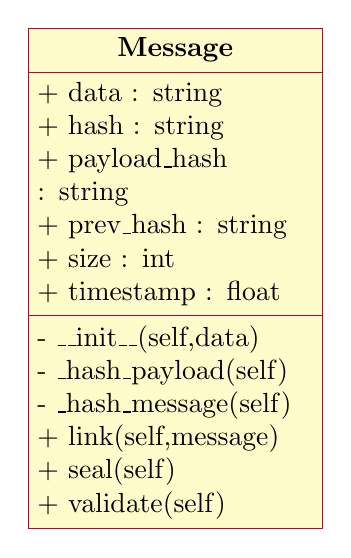
\begin{tikzpicture}			
				\begin{class}[text width = 3.5cm]{Message}{0, 0}
				\attribute{+ data : string}
				\attribute{+ hash : string}
				\attribute{+ payload\_hash : string}
				\attribute{+ prev\_hash : string}
				\attribute{+ size : int}
				\attribute{+ timestamp : float}
				
				\operation{- \_\_init\_\_(self,data)}
				\operation{- \_hash\_payload(self)}
				\operation{- \_hash\_message(self)}
				\operation{+ link(self,message)}
				\operation{+ seal(self)}
				\operation{+ validate(self)}
				\end{class}
				\end{tikzpicture}
			\end{center}				
		\end{figure}
	\end{minipage}%
\end{frame}

\subsection{区块的定义和实现}

\begin{frame}[fragile]
	\frametitle{区块的定义和实现}
	\begin{minipage}[t]{0.5\linewidth}
		\begin{itemize}
			\item 属性
			\begin{itemize}
				\item 消息的集合
				\item 当前块hash
				\item 前一个块hash
				\item 时间戳
			\end{itemize}
			\item 方法
			\begin{itemize}
				\item 添加消息
				\item 链接区块
				\item 生成区块哈希
				\item 验证区块完整性
			\end{itemize}
		\end{itemize}
	\end{minipage}%
	\begin{minipage}[t]{0.4\linewidth}
		\begin{figure}
		\begin{center}
			\scriptsize\ttfamily
			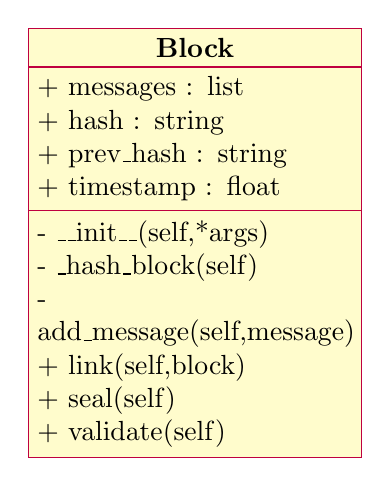
\begin{tikzpicture}			
			\begin{class}[text width = 4cm]{Block}{0, 0}
			\attribute{+ messages : list}
			\attribute{+ hash : string}
			\attribute{+ prev\_hash : string}
			\attribute{+ timestamp : float}
			
			\operation{- \_\_init\_\_(self,*args)}
			\operation{- \_hash\_block(self)}
			\operation{- add\_message(self,message)}
			\operation{+ link(self,block)}
			\operation{+ seal(self)}
			\operation{+ validate(self)}
			\end{class}
			\end{tikzpicture}
		\end{center}				
		\end{figure}
	\end{minipage}%
\end{frame}


\subsection{链的定义和实现}

\begin{frame}[fragile]
	\frametitle{链的定义和实现}
	\begin{minipage}[t]{0.5\linewidth}
		\begin{itemize}
			\item 属性
			\begin{itemize}
				\item 链的集合
			\end{itemize}
			\item 方法
			\begin{itemize}
				\item 添加区块
				\item 验证区块
			\end{itemize}
		\end{itemize}
	\end{minipage}%
	\begin{minipage}[t]{0.4\linewidth}
		\begin{figure}
			\begin{center}
				\scriptsize\ttfamily
				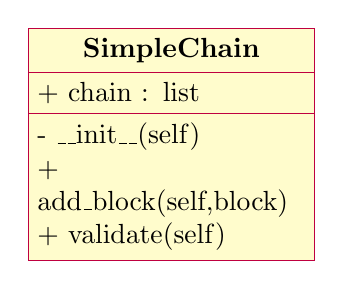
\begin{tikzpicture}			
				\begin{class}[text width = 3.4cm]{SimpleChain}{0, 0}
				\attribute{+ chain : list}
				
				\operation{- \_\_init\_\_(self)}
				\operation{+ add\_block(self,block)}
				\operation{+ validate(self)}
				\end{class}
				\end{tikzpicture}
			\end{center}				
		\end{figure}
	\end{minipage}%
\end{frame}




\subsection{业务逻辑的定义和实现}
\begin{frame}[fragile]
	\frametitle{业务逻辑的定义和实现}
	\begin{lstlisting}[basicstyle=\small\ttfamily]
区块链功能的基本实现,可以通过动作集对区块链进行操作。

动作集:
- 将消息添加到现有区块  (1)
- 将现有块添加到链      (2)
- 显示整个区块链        (3)
- 显示一个区块          (4)
- 验证区块链的完整性    (5)
- 退出程序              (6)

如果完整性受到威胁,则验证动作将终止程序。
\end{lstlisting}
\end{frame}

\subsection{运行简单区块链}

\begin{frame}[fragile]
	\frametitle{运行简单区块链}
在命令行输入下面的命令用docker运行打包好的环境:
		\begin{lstlisting}[language=sh,numbers=none,basicstyle=\fontsize{6}{7}\ttfamily]
docker run --rm -it registry.cn-shenzhen.aliyuncs.com/blockchain101/simpleblockcha1
\end{lstlisting}
\end{frame}

\section*{小结}
\begin{frame}
	\frametitle{实验课小结}
	\begin{itemize}
		\item 哈希可生成数据指纹,如消息的哈希:
		
		$hash_{message}=sha256(hash_{prev} + hash_{payload})$
		
		\item 哈希可以将消息、区块串联起来
		
		\item 消息和区块虽然类型不同但结构相似
	\end{itemize}
\end{frame}

\section*{附录}
\begin{frame}[allowframebreaks]{附录1:简单区块链源代码}
	\lstinputlisting[language=Python,basicstyle=\tiny,title="简单区块链源代码\cite{simplechaingithub}"]{./figures/simple_chain.py}
\end{frame}

\section*{参考文献}
\begin{frame}{参考资料}
	%	\printbibliography
	\bibliographystyle{plain}
	\bibliography{reference}
\end{frame}

\section*{谢谢聆听}

\begin{frame}
	\begin{minipage}[t]{0.5\linewidth}
		\begin{center}
			\begin{figure}
				\vspace{10pt}

				{\Huge 谢谢聆听}

				\vspace{30pt}
				郭泰彪

				\vspace{10pt}
				{\tiny 湖南工商大学大数据与互联网创新研究院}
			\end{figure}
			\begin{figure}

			\end{figure}
		\end{center}
	\end{minipage}%
	\begin{minipage}[t]{0.4\linewidth}
		\begin{figure}
			\centering
			\texttt{blockchain101}

			
\includegraphics[width=0.6\linewidth]{figures/blockchain101qrcode}

			{\footnotesize \texttt{Star| Fork| Issue}}
		\end{figure}
	\end{minipage}%
\end{frame}

\end{document}